\title{Aula 1 - Motivação Inicial}

\author{Prof. Gabriel Rodrigues Caldas de Aquino}

\institute
{
    Instituto de Computação \\
    Universidade Federal do Rio de Janeiro\\
    gabrielaquino@ic.ufrj.br % Your institution for the title page
}
\date{Compilado em: \\ \today} % Date, can be changed to a custom date

%----------------------------------------------------------------------------------------
%    PRESENTATION SLIDES
%----------------------------------------------------------------------------------------



\begin{frame}
    % Print the title page as the first slide
    \titlepage
\end{frame}

\begin{frame}{Preocupações da atualidade}
    \centering
    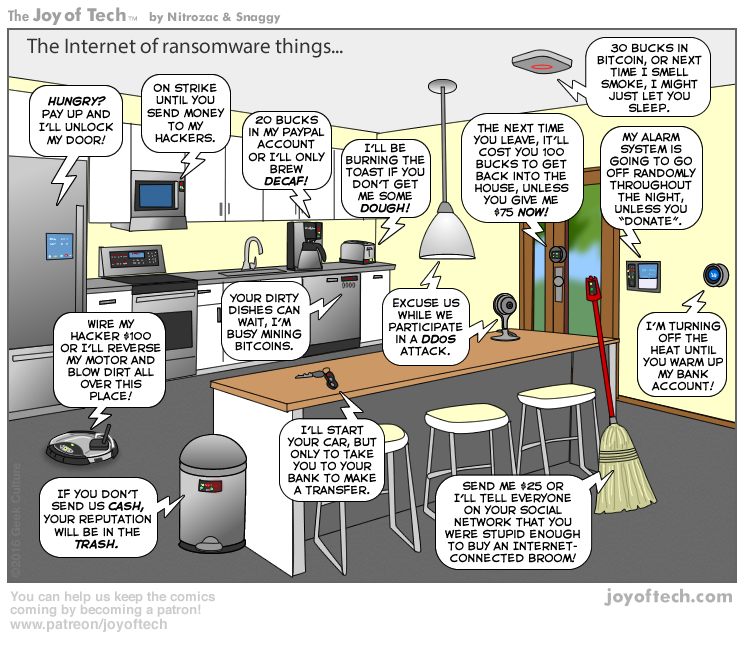
\includegraphics[width=0.63\linewidth]{Figuras/IoT-ransomware.png}


\end{frame}

\begin{frame}{Informação}

    \begin{block}{Ativo valioso}
        A informação é o ativo mais valioso para uma organização ou para uma pessoa.
    \end{block}

    \begin{exampleblock}{Por que?}
        \begin{itemize}
            \item \textbf{tomada de decisão}.
            \item \textbf{vantagem competitiva}.
            \item \textbf{ativo financeiro, estratégico ou pessoal}.
        \end{itemize}
    \end{exampleblock}

    \begin{alertblock}{Impactos da perda ou comprometimento}
        \begin{itemize}
            \item Prejuízos financeiros.
            \item Danos à reputação.
            \item Risco jurídico.
        \end{itemize}
    \end{alertblock}

\end{frame}

\begin{frame}{Preocupações da atualidade}
    \centering
    \begin{columns}
        \begin{column}{0.48\linewidth}
            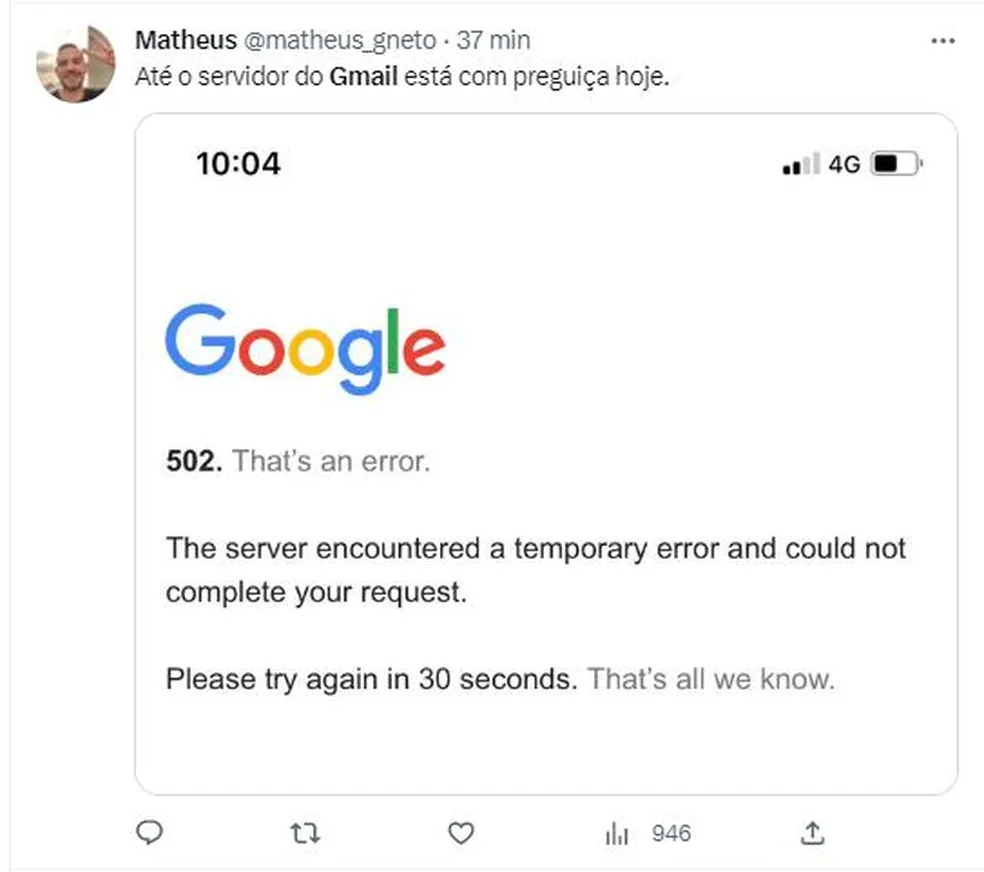
\includegraphics[width=\linewidth]{Figuras/gmail1.png}
        \end{column}
        \begin{column}{0.48\linewidth}
            
\includegraphics[width=\linewidth]{Figuras/gmail2.png}
        \end{column}
    \end{columns}
    \href{https://g1.globo.com/tecnologia/noticia/2023/02/27/gmail-e-outros-servicos-do-google-apresentam-instabilidade-nesta-segunda.ghtml}{Link: Notícia}
\end{frame}



\begin{frame}{Preocupações da atualidade}
    \centering
    \begin{columns}
        \begin{column}{0.48\linewidth}
            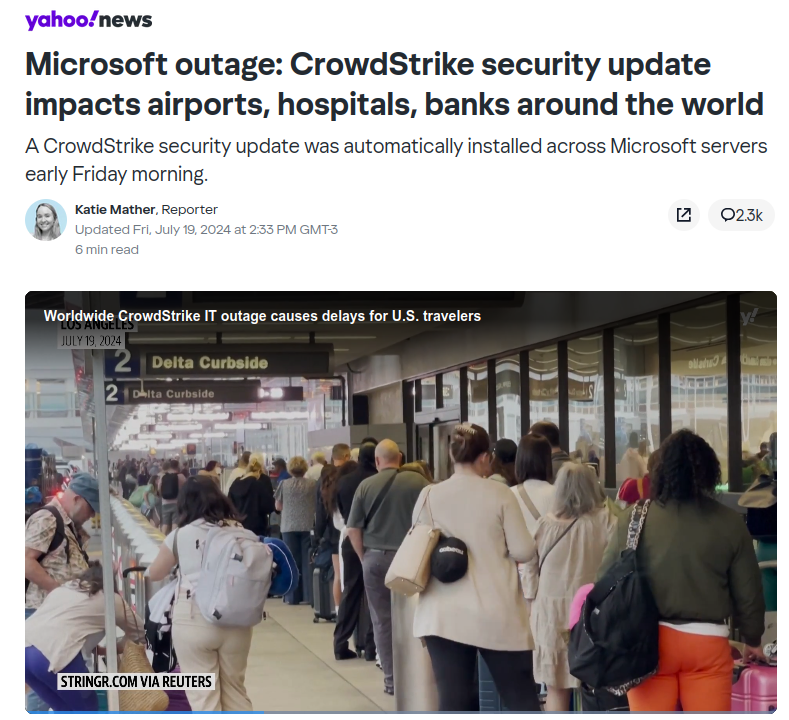
\includegraphics[width=\linewidth]{Figuras/crowdstrike1.png}
        \end{column}
        \begin{column}{0.48\linewidth}
            \includegraphics[width=\linewidth]{Figuras/crowdstrike2.png}
        \end{column}
    \end{columns}
    \href{https://www.yahoo.com/news/microsoft-outage-crowdstrike-security-update-impacts-airports-hospitals-banks-around-the-world-151137547.html}{Link: Notícia}
\end{frame}

\begin{frame}{Preocupações da atualidade}
    \centering
    \begin{columns}
        \begin{column}{0.48\linewidth}
            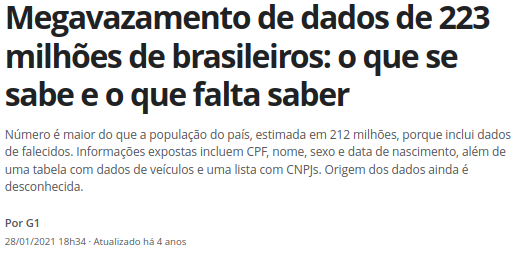
\includegraphics[width=\linewidth]{Figuras/megavazamento1.png}
            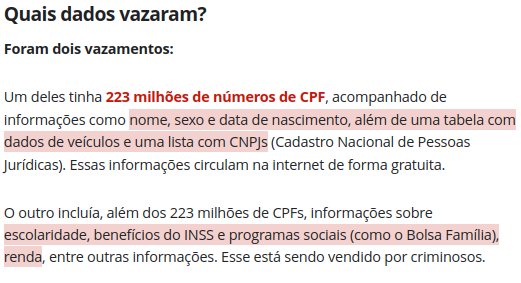
\includegraphics[width=\linewidth]{Figuras/megavazamento2.png}
        \end{column}
        \begin{column}{0.48\linewidth}
            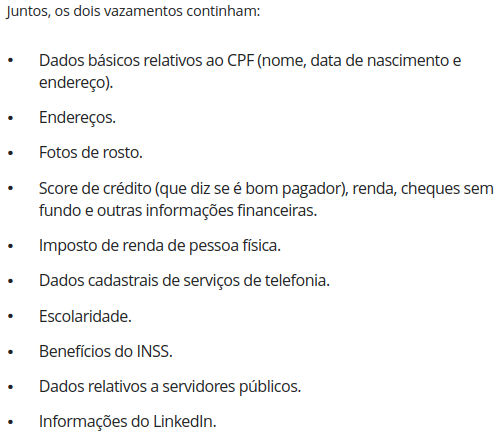
\includegraphics[width=\linewidth]{Figuras/megavazamento3.png}
        \end{column}
    \end{columns}
    \href{https://g1.globo.com/economia/tecnologia/noticia/2021/01/28/vazamento-de-dados-de-223-milhoes-de-brasileiros-o-que-se-sabe-e-o-que-falta-saber.ghtml}{Link: Notícia}

\end{frame}
\begin{frame}{Caso real brasileiro}

    \begin{block}{Caso Real no Brasil — 2025}
        \begin{itemize}
            \item Em julho de 2025, um ataque hacker contra a empresa C\&M Software resultou no desvio de cerca de \textbf{R\$541 milhões} de uma instituição financeira.

            \item C\&M Software provia a infraestrutura técnica para que seus clientes (bancos pequenos, fintechs, cooperativas de crédito, etc.) conseguissem se conectar ao Sistema de Pagamentos Instantâneos (SPI) e ao Sistema de Pagamentos Brasileiro (SPB) do Banco Central.
        \end{itemize}

    \end{block}

    \begin{block}{Repercussão na imprensa:}
        \href{https://www.cnnbrasil.com.br/nacional/brasil/ataque-hacker-o-que-sabemos-sobre-golpe-que-desviou-r-541-milhoes/}{Link 1} ;
        \href{https://g1.globo.com/sp/sao-paulo/noticia/2025/07/04/ataque-hacker-quem-e-suspeito-de-entregar-acesso-ao-sistema-que-liga-bancos-do-pix.ghtml}{Link 2} ;
        \href{https://cryptoid.com.br/ciberseguranca-seguranca-da-informacao/chaves-em-maos-erradas-licoes-do-maior-ataque-hacker-ao-sistema-financeiro/}{Link 3} ;
        \href{https://exame.com/insight/a-vida-apos-o-ataque-hacker-a-bmp-perdeu-r-500-milhoes-mas-resistiu-e-vai-virar-banco-multiplo/p}{link 4}

    \end{block}

    \begin{alertblock}{O que esse caso demonstra}
        \begin{itemize}
            \item Ataque que usou o fator humano ( "\textbf{insiders} confiáveis") - Fator humano é crítico.
            \item Uma única falha de segurança pode resultar em \textbf{prejuízos bilionários}.
        \end{itemize}
    \end{alertblock}

\end{frame}

\begin{frame}{Quanto Vale a Informação?}

    \begin{block}{Ideia central}
        O esforço despendido para proteger a informação depende diretamente do \textbf{valor dessa informação}.
    \end{block}

    \centering


    \vspace{0.5cm}

    \begin{alertblock}{Reflexão}
        Se a informação for \textbf{crítica} para o negócio ou para a vida das pessoas, a proteção deve ser proporcionalmente \textbf{robusta}.
    \end{alertblock}

\end{frame}

\begin{frame}{Quanto Vale a Informação?}

    \begin{block}{Princípio Econômico da Segurança da Informação}
        O custo para se proteger contra uma ameaça deve ser \textbf{menor} que o custo de recuperação caso a ameaça se concretize. RFC 2196
    \end{block}

    \href{https://datatracker.ietf.org/doc/html/rfc2196}{Link: RFC 2196 - Site Security Handbook}

    \vspace{0.5cm}

    \begin{alertblock}{Reflexão}
        Investir em segurança não é gasto — é evitar perdas maiores.
    \end{alertblock}

\end{frame}

\begin{frame}{Só que... no mundo real...}
    \centering
    \begin{columns}
        \begin{column}{0.48\linewidth}
            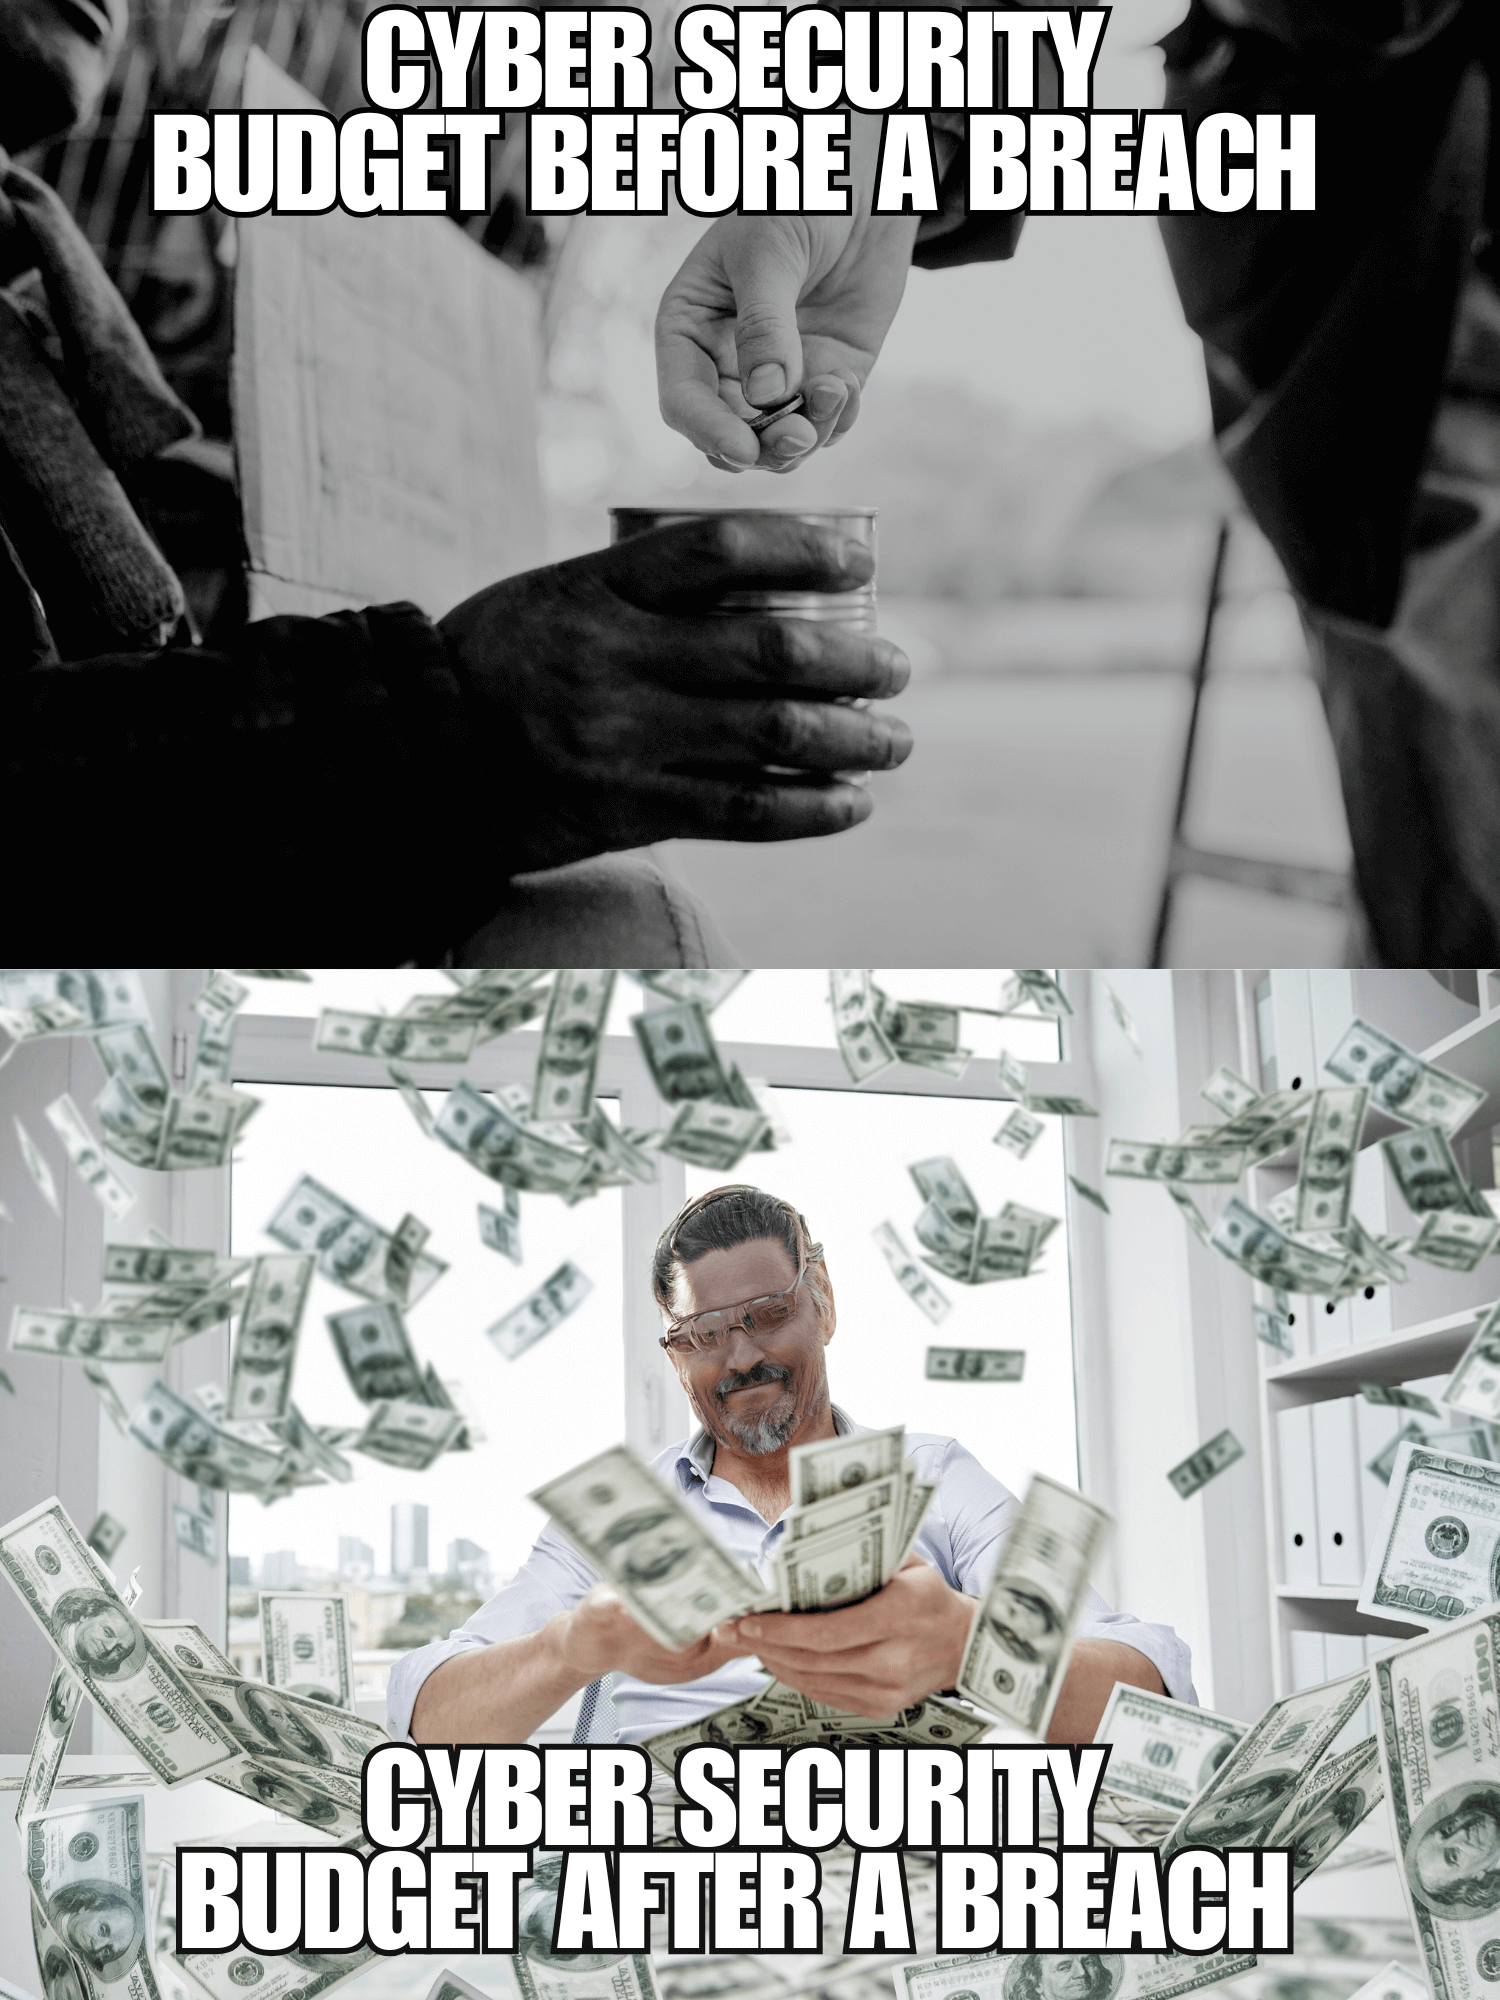
\includegraphics[width=0.8\linewidth]{Figuras/budget-seguranca-antes-depois.png}

        \end{column}
        \begin{column}{0.48\linewidth}
            
\includegraphics[width=\linewidth]{Figuras/empregado-clicou-errado.png}
        \end{column}
    \end{columns}


\end{frame}


